\documentclass[english]{article}
\usepackage[
 %work, %--- activate temporarily to visualise the type area while fine tuning the poster composition
 ,cursor
 ]{KITposter}
 
%Custom packages needed
\usepackage{siunitx}
\usepackage{pgfplots}
\pgfplotsset{compat=newest}
\usepgfplotslibrary{fillbetween}
\usepackage{tikzscale}
\usepackage{tabularx}
\usepackage{enumitem}
 
\title{Characterizing the Annoyance of the Nashville 2024 Cicada Population in the Time and Frequency Domain}
\author{\underline{M.-D. Noll}\thanks{marvin-dennis.noll@kit.edu}, O. Manzhura and M. Nabinger
}
\institute{}


\footline{\small%
\begin{tabularx}{\linewidth}{p{0.15\linewidth} X p{0.15\linewidth} p{0.09\linewidth}}
     \textbf{Contact} \newline
	 *Marvin-Dennis Noll -- \url{marvin-dennis.noll@kit.edu}\newline Institute for Beam Physics and Technology\newline\url{www.ibpt.kit.edu} \newline Karlsruhe, Germany &
	 \textbf{References} \newline
	 \begin{enumerate}[nosep,label={[}\arabic*{]}]
  \item \label{ref:3} University of Connecticut "The 2024 Periodical Cicada Emergence", https://cicadas.uconn.edu/ (visited on 21.05.2024)
	 \item \label{ref:1}S. Ozharar et al. "Long-term monitoring and analysis of Brood X cicada activity by distributed fiber optic sensing technology", 2023
  \item \label{ref:2} David C. Marshall and John R. Cooley "Reproductive Character Displacement and Speciation in Periodical Cicadas, with Description of a new Species, 13-Year Magicicada Neotredecim", 2000
	 \end{enumerate} &
	  \textbf{Acknowledgments} \newline 
	  M.-D. Noll acknowledges the support by the Doctoral School "Karlsruhe School of Elementary Particle and Astroparticle Physics: Science and Technology" and the ipac24 student grant &
	  \textbf{Conference} \newline
	  \raisebox{-4.5cm}{\begin{minipage}[t]{1cm}\includegraphics[width=8cm]{ipac24logoc}\\
	  \textbf{}\end{minipage}}\\
\end{tabularx}
}                          
            
\def\boxheight{200mm}           
\def\boxsep{6mm}     
\begin{document}
	\maketitle
	\vspace{-40mm}
	
	\begin{boxgrayw}[\boxheight]{Motivation}{}
		\begin{itemize}
			\item For the first time in 9 years a 13-year brood has emerged in the same year as a 17-year brood. \ref{ref:3}
            \item For the first time in 26 years adjacent 13-and 17-year broods will emerge in the same year. \ref{ref:3}
            \item The last time brood XIX and XIII co-emerged was over 200 years ago. In Nashville only Brood XIX can be seen. \ref{ref:3}
            \item It is possible to see all seven named periodical cicada species as adults in the same year. The next time this happens will be in 2037. \ref{ref:3}
		\end{itemize}
	\end{boxgrayw}
	\begin{boxgray2w}[\boxheight]{Time/Frequency Representation}{}
		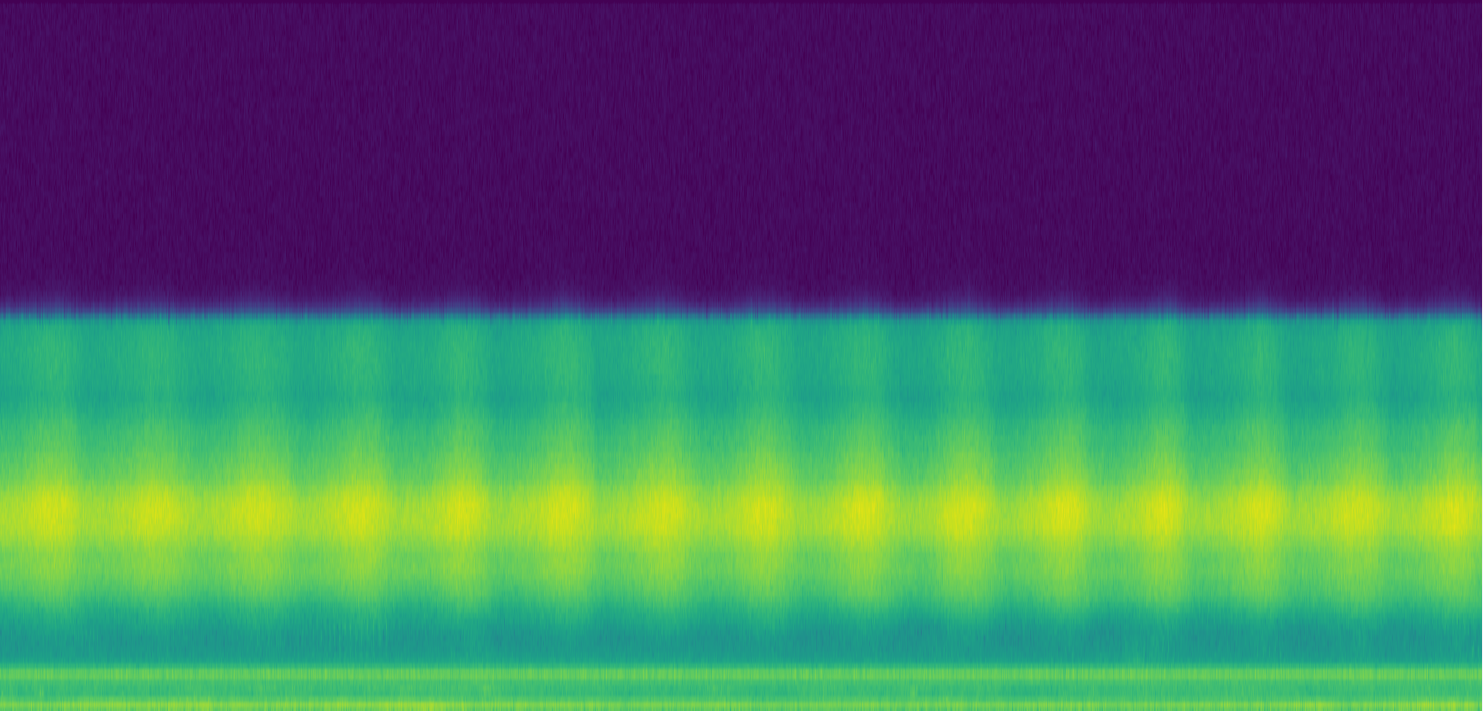
\includegraphics[height=175mm,width=470mm]{img/spect.tikz}
	\end{boxgray2w}
	\vskip\boxsep
	\begin{boxgray2w}[\boxheight]{Analysis in the Time Domain: Showing Rise/Decay of Audio Power}{}
		\includegraphics[height=175mm,width=460mm]{img/timesignal.tikz}
	\end{boxgray2w}
	\begin{boxgrayw}[\boxheight]{Captured Individuum}{}
		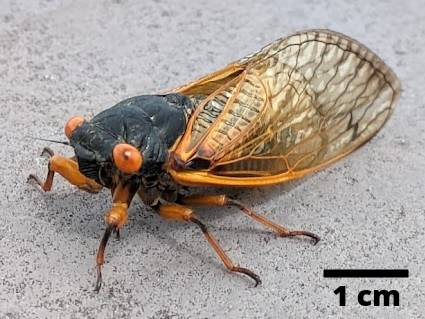
\includegraphics[width=205mm]{img/vieh2.png}
	\end{boxgrayw}
	\vskip\boxsep
	\begin{boxgray2w}[\boxheight]{Analysis in the Frequency Domain: Mean Frequency of Cicada Calls}{}
		\includegraphics[height=160mm,width=460mm]{img/period.tikz}
		The ensemble of cicada calls resemble a buzzing sound with 6 kHz center frequency
	\end{boxgray2w}
	\begin{boxgrayw}[\boxheight]{Outlook}{}
		\begin{itemize}
			\item The peak frequency of \SI{6}{\kilo \hertz} suggests that the species might be either \textit{M. cassini}, \textit{M. tredecassini}, \textit{M. septendecula} or \textit{M. tredecula} (according to \ref{ref:2})
            \item Further investigations need to be conducted, preferrably with better audio equipment, in order to pin-point the exact peak frequencies of the cicada chorus.
            \item Spending too much time in nature, as long as the cicadas are alive, might damage your hearing permanently.
		\end{itemize}
	\end{boxgrayw}
\end{document}
